%%%%%%%%%%%%%%%%%%%%%%%%%%%%%%%%%%%%%%%%%
% Poster V14 — Energy Aware Computing Continuum
% Updated with new energy-objective results (Greedy-E / CSP / LLM no seeds)
% Color scheme: original template (pink headers, green taxonomy, orange benchmark)
% Layout: Right column = Results → Conclusion → References (top to bottom)
%%%%%%%%%%%%%%%%%%%%%%%%%%%%%%%%%%%%%%%%%

\documentclass[a0paper,portrait]{baposter}

\usepackage[font=small,labelfont=bf]{caption}
\usepackage{booktabs}
\usepackage{relsize}
\usepackage{helvet}
\renewcommand{\familydefault}{\sfdefault}
\usepackage{amsmath,amsfonts,amssymb}
\usepackage{textcomp}
\usepackage{tikz}
\usetikzlibrary{arrows.meta,positioning,fit,backgrounds,calc}
\usepackage{colortbl}
\usepackage{xcolor}
\usepackage{enumitem}

\graphicspath{{figures/}}

%--- COLORS (same as original template) ---
\definecolor{bordercol}{RGB}{80,80,80}
\definecolor{esilvcol}{RGB}{206,16,82}
\definecolor{headercol1}{RGB}{230,100,150}    % pink — default headers
\definecolor{headercol2}{RGB}{230,100,150}
\definecolor{headerfontcol}{RGB}{255,255,255}
\definecolor{boxcolor}{RGB}{250,250,248}
\definecolor{bgcol}{RGB}{252,252,250}
\definecolor{taxonomycol}{RGB}{100,180,100}   % green — taxonomy
\definecolor{benchmarkcol}{RGB}{240,140,60}   % orange — benchmarking / results
\definecolor{bestrow}{RGB}{255,230,210}       % green-tinted for table highlight

% Taxonomy radial diagram: 4 soft dims
\definecolor{coreCol}{RGB}{206,16,82}
\definecolor{dimA}{RGB}{70,120,190}
\definecolor{dimAlight}{RGB}{225,235,252}
\definecolor{dimB}{RGB}{80,160,90}
\definecolor{dimBlight}{RGB}{225,248,228}
\definecolor{dimC}{RGB}{160,105,50}
\definecolor{dimClight}{RGB}{252,242,225}
\definecolor{dimD}{RGB}{130,80,155}
\definecolor{dimDlight}{RGB}{242,232,252}

% Infra tiers
\definecolor{tiercloud}{RGB}{70,120,190}
\definecolor{tierfog}{RGB}{160,120,50}
\definecolor{tieredge}{RGB}{80,160,90}
\definecolor{neutral}{RGB}{100,100,105}
\definecolor{neutrallight}{RGB}{242,242,244}

% Accent for inline labels
\definecolor{labelcol}{RGB}{60,60,65}

\begin{document}

\background{
\begin{tikzpicture}[remember picture,overlay]
  \fill[bgcol] (current page.south west) rectangle (current page.north east);
\end{tikzpicture}
}

\begin{poster}{
  grid=false, columns=6,
  borderColor=bordercol,
  headerColorOne=headercol1, headerColorTwo=headercol2,
  headerFontColor=headerfontcol,
  boxColorOne=boxcolor,
  headershape=roundedright, headerfont=\Large\sf\bf,
  textborder=rectangle, background=user,
  headerborder=open, boxshade=plain
}
{\includegraphics[width=0.1\textwidth]{esilv.png}}
{\centering \bf \huge {Energy-Aware Computing Continuum} \\[6pt]
 \Large \it Taxonomy, Modeling and Optimization of Energy in Cloud-Edge Infrastructures}
{\centering \vspace{0.4em} \smaller {\bf Théo HARDY}$^{1}$, Farah Aït Salaht$^{1}$, Daniel WLADDIMIRO$^{1}$ \\[2pt]
\smaller $^{1}$\it {ESILV -- De Vinci Research Center (DVRC)} \\}
{\includegraphics[width=0.15\textwidth]{dvrc.png}}

%========================================================================================
%   ROW 1 — CONTEXT & PROBLEM (full width, default pink header)
%========================================================================================
\headerbox{Context \& Problem Statement}{name=intro,column=0,row=0,span=6}{
\begin{minipage}{0.63\linewidth}
\textbf{\textcolor{esilvcol}{Context.}}
The Cloud-Edge Computing Continuum (CECC) integrates IoT devices, edge/fog nodes, and cloud data centers into a unified infrastructure.
It enables multi-service deployment closer to users, but \textit{where to place each component to minimize energy under QoS constraints?}

\vspace{3mm}

\textbf{\textcolor{esilvcol}{Problem.}}
Energy modeling across the CECC is \textbf{fragmented}: formulations, scopes, and methods vary widely.
Most strategies optimize latency or cost, rarely a \textbf{unified energy objective} covering nodes \textit{and} network.
\end{minipage}%
\hfill
\begin{minipage}{0.34\linewidth}
  \centering
  \includegraphics[width=.7\linewidth, trim={1.2cm 1.5cm 1.2cm 1.5cm}, clip]{Cloud_Fog_Edge_scheme}
\end{minipage}
}

%========================================================================================
%   ROW 2 — CONTRIBUTIONS (full width, default pink header)
%========================================================================================
\headerbox{Contributions}{name=contrib,column=0,span=6,below=intro}{

\begin{minipage}{0.48\linewidth}
\colorbox{taxonomycol!15}{\parbox{0.95\linewidth}{%
\textbf{\textcolor{taxonomycol}{Phase 1 : Review \& Taxonomy}}\\[2pt]
\textit{Who} consumes \textit{what}, \textit{which models}, \textit{how} measured.\\
$\rightarrow$ \textbf{4-dimension taxonomy} (scope, decomposition, abstraction, methodology).%
}}
\end{minipage}%
\hfill
\begin{minipage}{0.48\linewidth}
\colorbox{benchmarkcol!15}{\parbox{0.95\linewidth}{%
\textbf{\textcolor{benchmarkcol}{Phase 2 : Energy-Aware Placement}}\\[2pt]
{\bf Unified energy objective:} $\min E_{\text{nodes}} + E_{\text{links}}$.
3 Python solvers: \textbf{Greedy-E} (FFD energy), \textbf{CSP} (CP-SAT), \textbf{LLM} (OPRO, Llama~3.1 local, no seed hints).%
}}
\end{minipage}

}

%========================================================================================
%   LEFT — TAXONOMY (green header)
%========================================================================================
{\colorlet{headercol1}{taxonomycol}\colorlet{headercol2}{taxonomycol}
\headerbox{\textcolor{white}{Taxonomy \& Synthesis}}{name=taxonomy,column=0,span=3,below=contrib}{

\begin{center}
\resizebox{0.98\linewidth}{!}{%
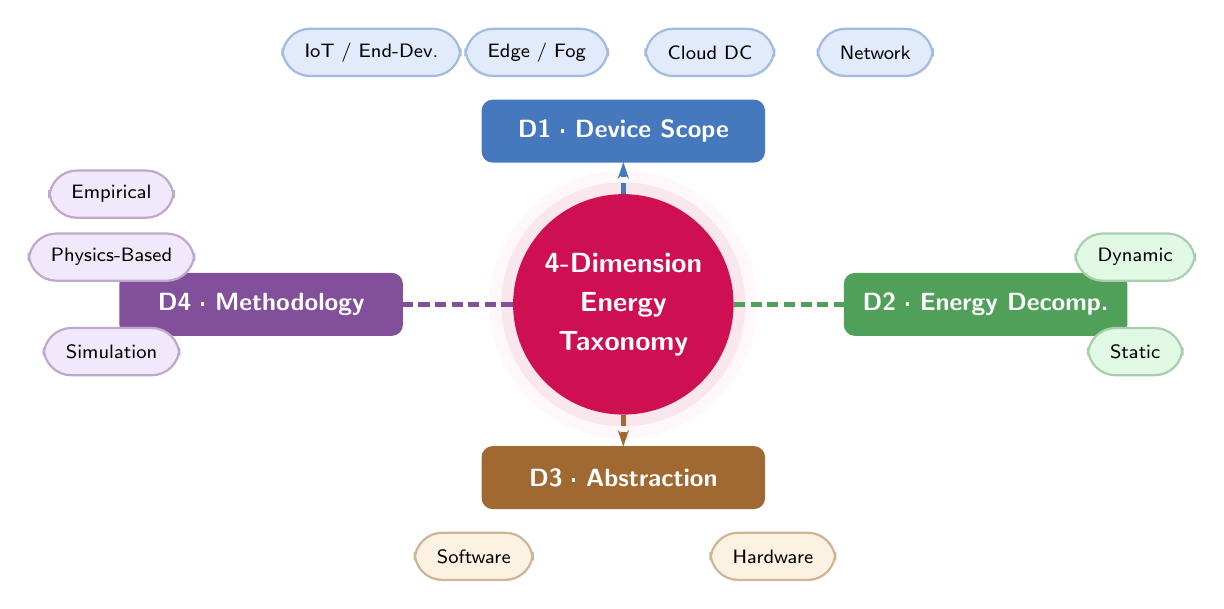
\begin{tikzpicture}[
  every node/.style={font=\sffamily},
  corecircle/.style={circle, minimum size=2.8cm, fill=coreCol, text=white,
    font=\sffamily\bfseries\normalsize, align=center, inner sep=0pt},
  dimheader/.style n args={1}{rounded corners=4pt, minimum height=0.8cm, minimum width=3.6cm,
    font=\sffamily\bfseries\small, text=white, align=center, fill=#1, inner sep=4pt},
  tag/.style n args={2}{draw=#1, fill=#2, rounded corners=10pt,
    minimum height=0.6cm, inner xsep=8pt, font=\sffamily\scriptsize, thick, align=center},
  connline/.style n args={1}{line width=2pt, color=#1, dash pattern=on 4pt off 2pt,
    -{Stealth[length=6pt, width=4pt]}},
]
\begin{scope}[on background layer]
  \fill[coreCol!3] (0,0) circle (1.7cm);
\end{scope}
\fill[coreCol!10] (0,0) circle (1.55cm);
\node[corecircle] (core) {4-Dimension\\[2pt]Energy\\[2pt]Taxonomy};
% D1 TOP
\draw[connline={dimA}] (core.north) -- ++(0, 0.4);
\node[dimheader={dimA}] (d1h) at (0, 2.2) {D1 \textperiodcentered\ Device Scope};
\node[tag={dimA!50}{dimAlight}] at (-3.2, 3.2) {IoT / End-Dev.};
\node[tag={dimA!50}{dimAlight}] at (-1.1, 3.2) {Edge / Fog};
\node[tag={dimA!50}{dimAlight}] at ( 1.1, 3.2) {Cloud DC};
\node[tag={dimA!50}{dimAlight}] at ( 3.2, 3.2) {Network};
% D2 RIGHT
\draw[connline={dimB}] (core.east) -- ++(1.8, 0);
\node[dimheader={dimB}] (d2h) at (4.6, 0) {D2 \textperiodcentered\ Energy Decomp.};
\node[tag={dimB!50}{dimBlight}] at (6.5,  0.6) {Dynamic};
\node[tag={dimB!50}{dimBlight}] at (6.5, -0.6) {Static};
% D3 BOTTOM
\draw[connline={dimC}] (core.south) -- ++(0, -0.4);
\node[dimheader={dimC}] (d3h) at (0, -2.2) {D3 \textperiodcentered\ Abstraction};
\node[tag={dimC!50}{dimClight}] at (-1.9, -3.2) {Software};
\node[tag={dimC!50}{dimClight}] at ( 1.9, -3.2) {Hardware};
% D4 LEFT
\draw[connline={dimD}] (core.west) -- ++(-1.8, 0);
\node[dimheader={dimD}] (d4h) at (-4.6, 0) {D4 \textperiodcentered\ Methodology};
\node[tag={dimD!50}{dimDlight}] at (-6.5,  1.4) {Empirical};
\node[tag={dimD!50}{dimDlight}] at (-6.5,  0.6) {Physics-Based};
\node[tag={dimD!50}{dimDlight}] at (-6.5, -0.6) {Simulation};
\end{tikzpicture}
}%
\end{center}

\textcolor{labelcol}{\textbf{Operational Energy Formulations:}}
\vspace{-0.15cm}
\begin{itemize}[leftmargin=*, itemsep=-2pt]
  \item \textbf{Server:} $P_{\text{idle}} + (P_{\text{max}} - P_{\text{idle}}) \cdot u$ \enspace (linear CPU)
  \item \textbf{Data Center:} Adds cooling via PUE factor
  \item \textbf{Communication:} $\propto bw \times lat^2$ per network link
  \item \textbf{State-Based:} Power over idle/active states
\end{itemize}

\textcolor{labelcol}{\textbf{Energy-Aware Placement \& Validation:}}
Design of placement algorithms optimizing energy, validated through Python simulations and real deployment on GCP VMs with Apache Storm.

}}

%========================================================================================
%   LEFT — BENCHMARKING (orange header, anchored to bottom)
%========================================================================================
{\colorlet{headercol1}{benchmarkcol}\colorlet{headercol2}{benchmarkcol}
\headerbox{\textcolor{white}{Benchmarking: Case Study}}{name=bench,span=3,column=0,below=taxonomy,above=bottom}{

\small

\begin{center}
\textbf{8-Node CECC Infrastructure \quad\&\quad 4-Component DSP Application}
\end{center}

\vspace{-0.1cm}

\begin{minipage}[t]{0.62\linewidth}
\centering
{\footnotesize\textbf{Infrastructure} (Cloud / Fog / Edge)}

\vspace{0.1cm}

\resizebox{\linewidth}{!}{%
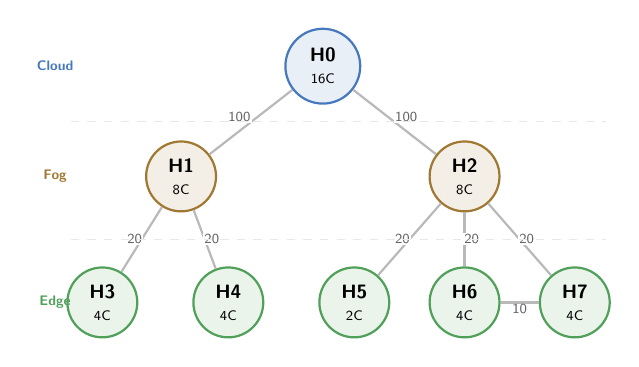
\begin{tikzpicture}[
  every node/.style={font=\sffamily\scriptsize},
  cloudN/.style={circle, draw=tiercloud, fill=tiercloud!12, thick, minimum size=0.95cm, align=center},
  fogN/.style={circle, draw=tierfog, fill=tierfog!12, thick, minimum size=0.85cm, align=center},
  edgeN/.style={circle, draw=tieredge, fill=tieredge!12, thick, minimum size=0.75cm, align=center},
  link/.style={neutral!45, thick},
  ll/.style={font=\sffamily\tiny, text=neutral, midway, fill=white, inner sep=0.5pt},
]
\node[cloudN] (h0) at (2.8, 3.8) {\textbf{H0}\\{\tiny 16C}};
\node[fogN] (h1) at (1.0, 2.4) {\textbf{H1}\\{\tiny 8C}};
\node[fogN] (h2) at (4.6, 2.4) {\textbf{H2}\\{\tiny 8C}};
\node[edgeN] (h3) at (0, 0.8) {\textbf{H3}\\{\tiny 4C}};
\node[edgeN] (h4) at (1.6, 0.8) {\textbf{H4}\\{\tiny 4C}};
\node[edgeN] (h5) at (3.2, 0.8) {\textbf{H5}\\{\tiny 2C}};
\node[edgeN] (h6) at (4.6, 0.8) {\textbf{H6}\\{\tiny 4C}};
\node[edgeN] (h7) at (6.0, 0.8) {\textbf{H7}\\{\tiny 4C}};
\draw[link] (h0) -- node[ll, above left=-1pt] {100} (h1);
\draw[link] (h0) -- node[ll, above right=-1pt] {100} (h2);
\draw[link] (h1) -- node[ll, left=-1pt] {20} (h3);
\draw[link] (h1) -- node[ll, right=-1pt] {20} (h4);
\draw[link] (h2) -- node[ll, left=-1pt] {20} (h5);
\draw[link] (h2) -- node[ll, right=-1pt] {20} (h6);
\draw[link] (h2) -- node[ll, right=-1pt] {20} (h7);
\draw[link] (h6) -- node[ll, below] {10} (h7);
\draw[dashed, neutral!15] (-0.4, 3.1) -- (6.4, 3.1);
\draw[dashed, neutral!15] (-0.4, 1.6) -- (6.4, 1.6);
\node[font=\sffamily\tiny\bfseries, text=tiercloud] at (-0.6, 3.8) {Cloud};
\node[font=\sffamily\tiny\bfseries, text=tierfog] at (-0.6, 2.4) {Fog};
\node[font=\sffamily\tiny\bfseries, text=tieredge] at (-0.6, 0.8) {Edge};
\end{tikzpicture}
}%
\end{minipage}%
\hfill
\begin{minipage}[t]{0.34\linewidth}
\centering
{\footnotesize\textbf{Application DAG}}

\vspace{0.1cm}

\resizebox{0.55\linewidth}{!}{%
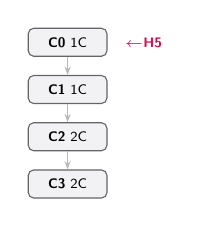
\begin{tikzpicture}[
  every node/.style={font=\sffamily\tiny},
  comp/.style={rounded corners=2pt, draw=neutral, minimum width=1.0cm, minimum height=0.35cm, align=center, fill=neutrallight},
  arr/.style={-{Stealth[length=3pt]}, neutral!45},
]
\node[comp] (c0) at (0, 1.8) {\textbf{C0} 1C};
\node[comp] (c1) at (0, 1.2) {\textbf{C1} 1C};
\node[comp] (c2) at (0, 0.6) {\textbf{C2} 2C};
\node[comp] (c3) at (0, 0.0) {\textbf{C3} 2C};
\draw[arr] (c0) -- (c1);
\draw[arr] (c1) -- (c2);
\draw[arr] (c2) -- (c3);
\node[font=\sffamily\tiny\bfseries, text=esilvcol, anchor=west] at (0.6, 1.8) {$\leftarrow$H5};
\end{tikzpicture}
}%

\end{minipage}

\begin{center}
\colorbox{benchmarkcol!12}{\parbox{0.90\linewidth}{\centering\footnotesize%
\textbf{Objective:} minimize $E_{\text{total}} = \underbrace{E_{\text{nodes}}}_{\sum P_{\text{idle}} + cpu_j \cdot 5} + \underbrace{E_{\text{links}}}_{\sum bw_l \cdot lat^2}$
\\ s.t.\ CPU, RAM, BW, latency, DZ constraints.%
}}
\end{center}

\vspace{-0.1cm}

\textcolor{labelcol}{\textbf{Placement Strategies (all minimizing energy):}}
\vspace{-0.1cm}
\begin{itemize}[leftmargin=*, itemsep=-2pt]
\item \textbf{Greedy-E (FFD):} sorts by CPU demand, places on the host minimizing $\Delta E_{\text{total}}$.
  \item \textbf{CSP (CP-SAT):} exact solver (OR-Tools), provably optimal for $E_{\text{total}}$.
  \item \textbf{LLM (Llama~3.1, local):} OPRO-style iterative prompting, 8 rounds, \textbf{no seed placements} (pure LLM exploration).
\end{itemize}

\vspace{0.1cm}

\textcolor{labelcol}{\textbf{Why compare these three?}}
Greedy-E is fast but myopic; CSP is optimal but may not scale.
LLMs offer a \textbf{flexible} alternative, but \textit{can they match CSP quality without heuristic hints, and at what energy cost?}

}}

%========================================================================================
%   RIGHT — PRELIMINARY RESULTS (orange header, below contrib)
%========================================================================================
{\colorlet{headercol1}{benchmarkcol}\colorlet{headercol2}{benchmarkcol}
\headerbox{\textcolor{white}{Preliminary Results}}{name=results,span=3,column=3,below=contrib}{

\begin{center}
\textcolor{labelcol}{\textbf{Greedy-E vs.\ CSP vs.\ LLM}}
\end{center}

\vspace{-6mm}

{\small
\begin{center}
\begin{tabular}{l|c|>{\columncolor{benchmarkcol!12}}c|c}
\toprule
\textbf{Metric} & \textbf{Greedy-E (FFD)} & \textbf{CSP (Optimal)} & \textbf{LLM (Llama\,3.1)} \\
\midrule
$E_{\text{total}}$          & 4\,160\,430 & \textbf{160\,430} & 4\,160\,430 \\
$E_{\text{links}}$          & 4\,160\,000 & \textbf{160\,000} & 4\,160\,000 \\
$E_{\text{nodes}}$          & 430      & 430               & 430               \\
Latency $e2e$ (ms)          & 120      & \textbf{20}       & 120               \\
Solve time                   & $<$0.001\,s & 0.19\,s        & 18.2\,s           \\
Tokens (in+out)              &,      &,               & 8\,338            \\
$E_{\text{solver}}$ (Wh)    & $\approx$0 & 0.002           & 0.228             \\
\bottomrule
\end{tabular}
\end{center}
}

\vspace{0.1cm}

\colorbox{benchmarkcol!12}{\parbox{0.95\linewidth}{\centering%
{\small  CSP achieves \textbf{--96\% energy} vs.\ Greedy-E ($160$k vs.\ $4.16$M), latency $\div$6.
  \textbf{LLM converges to the same suboptimal placement as Greedy-E}:
  all free components on H0~(cloud) instead of H2~(fog, near DZ host H5).
  $E_{\text{links}}$ dominates ($>$99.99\% of $E_{\text{total}}$): \textbf{host proximity is the key factor.}%
}}}

\vspace{0.15cm}

%\colorbox{benchmarkcol!12}
{\parbox{0.95\linewidth}{\footnotesize%
\textbf{Solver energy model:} \enspace
$E_{\text{solver}} = P_{\text{device}} \times T_{\text{inference}}$
\enspace where \enspace
$T_{\text{inference}} \propto N_{\text{tokens}} / \text{throughput}$\\[2pt]
\textbf{Goal:} integrate $E_{\text{solver}}$ into the placement objective:
\enspace $\min\; E_{\text{total}} + E_{\text{solver}}$%
}
}

\vspace{0.15cm}

\colorbox{taxonomycol!12}{\parbox{0.95\linewidth}{\footnotesize%
\textbf{Energy ROI of the solver:} \enspace
$\text{ROI}_E = \dfrac{\Delta E_{\text{placement}}}{E_{\text{solver}}}$
\\[4pt]
\begin{tabular}{l|c|c}
 & \textbf{CSP} & \textbf{LLM (Llama\,3.1)} \\
\hline
$\Delta E_{\text{placement}}$ & 4\,000\,000 & 0 \\
$E_{\text{solver}}$ (Wh) & 0.002 & 0.228 \\
$\text{ROI}_E$ & $1.69 \times 10^{9}$ & 0 (no gain) \\
%$T^{*}$ (payback) & $\approx 0$\,s & never \\
\end{tabular}\\[3pt]
\textbf{$\Rightarrow$ CSP pays back instantly} ($\Delta E = 4$M, solver cost negligible). 
LLM (no seeds): \textbf{same result as Greedy-E}, 8\,338 tokens consumed for zero energy gain.%
}}

}}

%========================================================================================
%   RIGHT — CONCLUSION (default pink header, below results)
%========================================================================================
\headerbox{Conclusion \& Future Work}{name=conclusion,column=3,below=results,span=3}{

\colorbox{esilvcol!10}{\parbox{0.96\linewidth}{%
\textbf{\textcolor{esilvcol}{Key Contributions}}\\[3pt]
{\small\textbullet~\textbf{4-dimension energy taxonomy} for the Cloud-Edge continuum.\\[2pt]
\textbullet~\textbf{Unified energy benchmark} (Greedy-E / CSP / LLM) with energy objective; first validation on GCP.
}}}

\vspace{0.25cm}

\textcolor{labelcol}{\textbf{Two papers in progress:}}
{\small
\vspace{0.1cm}
\begin{itemize}[leftmargin=*, itemsep=-2pt]
  \item \textbf{COMPAS 2025:} \textit{``Heuristic, CSP or LLM? Comparative Study of the Energy Cost of Service Placement in the Cloud.''}
  \item \textbf{Journal (mini-survey):} Energy aspects in the CECC, models, formulations, measurement across Cloud-Edge tiers.
\end{itemize}

\vspace{-0.1cm}

\textcolor{labelcol}{\textbf{Perspectives:}}
%\vspace{0.1cm}
\begin{itemize}[leftmargin=*, itemsep=-2pt]
  \item Scaling study on \textbf{larger instances} where CSP may time out and LLM could shine.
%  \item Test LLM \textbf{with seed hints} vs.\ without, to quantify the value of heuristic guidance.
  \item Deploy solvers in the \textbf{GCP Storm scheduler} for live workload validation.
\end{itemize}}
}

%========================================================================================
%   RIGHT — REFERENCES (default pink header, below conclusion, anchored to bottom)
%========================================================================================
\headerbox{References}{name=references,column=3,below=conclusion,above=bottom,span=3}{
\smaller
\begin{enumerate}[leftmargin=*, label={[\arabic*]}, itemsep=1pt]
\item F. Ait Salaht, et al. "Service placement in fog computing using constraint programming." SCC. IEEE, 2019.\vspace{-1mm}
  \item A.~Beloglazov, et al. \textit{Optimal online algorithms for energy minimization in large-scale cloud}. IEEE TPDS, 2012.\vspace{-1mm}
  \item C.~Yang et al. \textit{Large Language Models as Optimizers}. ICLR, 2024 (OPRO).
\end{enumerate}
}

\end{poster}
\end{document}
